\documentclass{article}
\usepackage[UTF8]{ctex}
\usepackage{pythonhighlight}
\usepackage{listings}
\lstset{
    basicstyle          =   \tt,          % 基本代码风格
    identifierstyle=\color{brown!80!black},
    keywordstyle        =   \color{purple}\bfseries,          % 关键字风格
    commentstyle        =   \rmfamily\itshape,  % 注释的风格,斜体
    stringstyle         =   \ttfamily,  % 字符串风格
    flexiblecolumns,                % 别问为什么,加上这个
    numbers             =   left,   % 行号的位置在左边
    showspaces          =   false,  % 是否显示空格,显示了有点乱,所以不现实了
    numberstyle         =   \zihao{-5}\ttfamily,    % 行号的样式,小五号,tt等宽字体
    showstringspaces    =   false,
    captionpos          =   t,      % 这段代码的名字所呈现的位置,t指的是top上面
    frame               =   lrtb,   % 显示边框
    backgroundcolor=\color[RGB]{245,245,244},
}
% Language setting
% Replace `english' with e.g. `spanish' to change the document language
\usepackage[english]{babel}
\usepackage{float}
% Set page size and margins
% Replace `letterpaper' with `a4paper' for UK/EU standard size
\usepackage[letterpaper,top=2cm,bottom=2cm,left=3cm,right=3cm,marginparwidth=1.75cm]{geometry}

% Useful packages
\usepackage{amsmath}
\usepackage{graphicx}
\usepackage[colorlinks=true, allcolors=blue]{hyperref}

% 标题、日期、作者信息在前面
\title{数据库实验报告2}
\author{雷远航 / 3210105807}
\date{2023.3.11}


\begin{document}

%\tableofcontents
% 可用于目录的生成


\maketitle


\begin{abstract}
    实验二: SQL 数据定义和操作
\end{abstract}

\section{实验目的}
    \subsection*{- 掌握关系数据库语言 SQL 的使用}
    \subsection*{- 使所有的 SQL 作业都能上机通过}

\section{实验平台}
    \subsection*{MySQL}

\section{内容和要求}
    \subsection*{- 建立数据库。}
    \subsection*{- 数据定义: 表的建立/删除/修改; 索引的建立/删除;视图的建立/删除}
    \subsection*{- 数据更新: 用 insert/delete/update 命令插入/删除/修改表数据。}
    \subsection*{- 数据查询: 单表查询,多表查询, 嵌套子查询等。}
    \subsection*{- 视图操作:通过视图的数据查询和数据修改}
    \subsection*{- 所有的 SQL 作业都上机通过}


\section{实验过程}

\subsection*{创建一个表}

首先创建一张表:

在数据库 COMPANY 中创建一个 employee 的表

\begin{figure}[H]
    \centering
    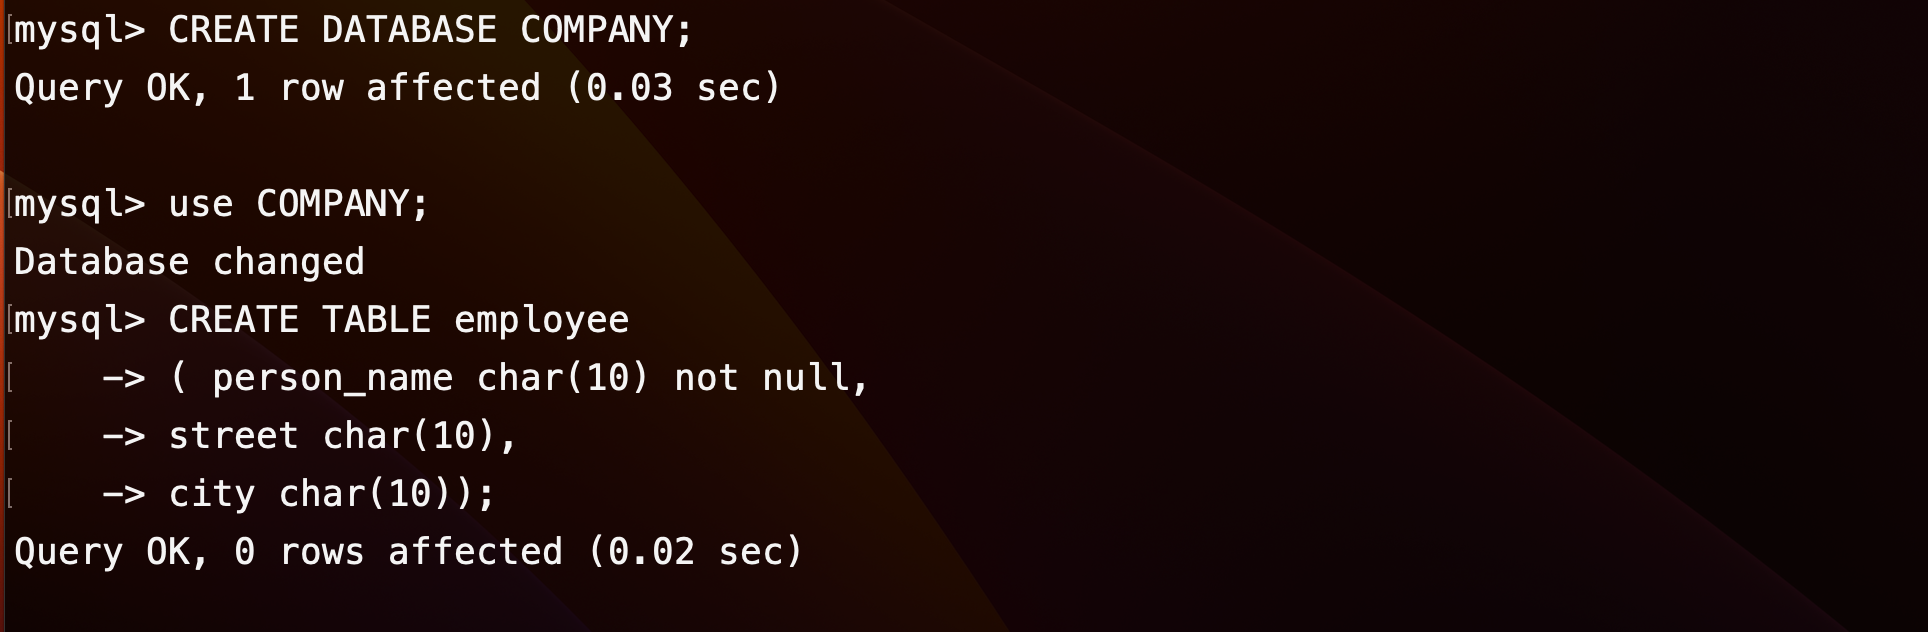
\includegraphics[width=1\textwidth]{lab2/1.png}
    \end{figure}


\subsection*{表的修改和删除}

使用 `ALTER` 进行表的修改

使用 `DROP` 进行表的删除

\begin{figure}[H]
    \centering
    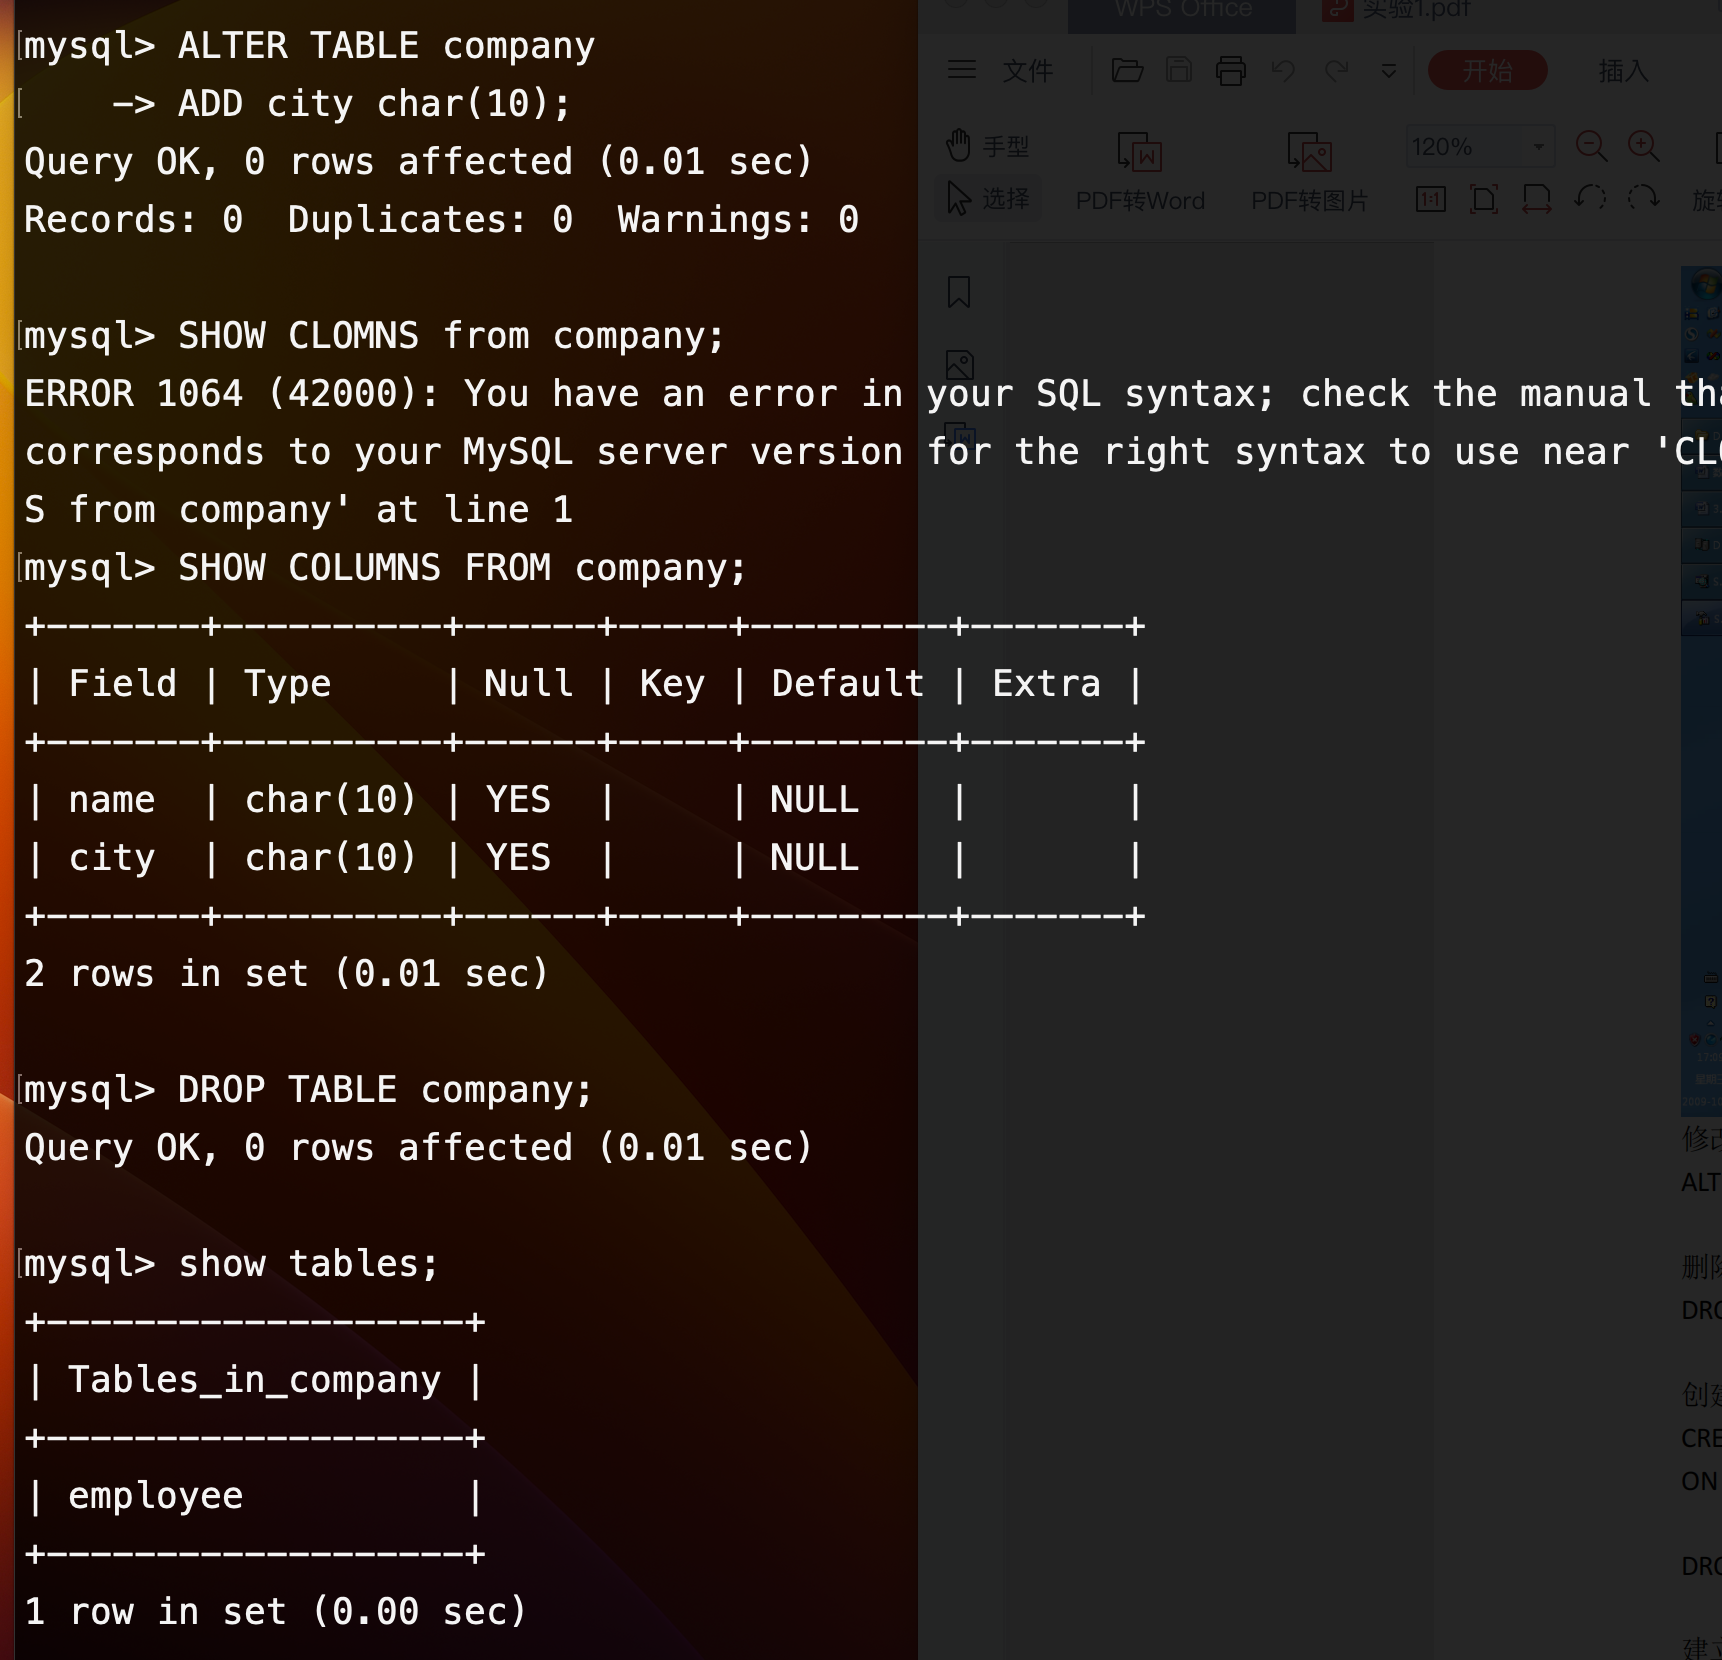
\includegraphics[width=1\textwidth]{lab2/2.png}
    \end{figure}


\subsection*{创建/删除索引}

创建以及删除索引的过程如下

\begin{figure}[H]
    \centering
    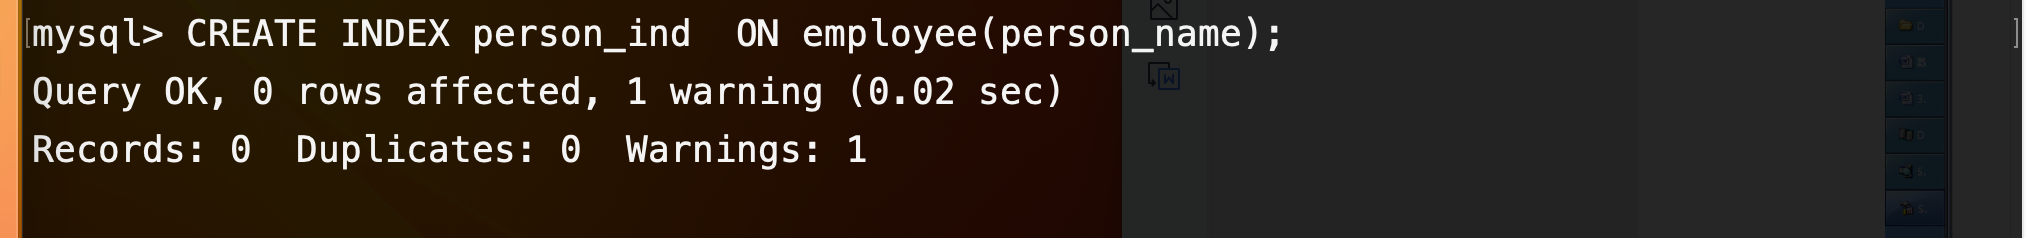
\includegraphics[width=1\textwidth]{lab2/3.png}
    \end{figure}


    \begin{figure}[H]
        \centering
        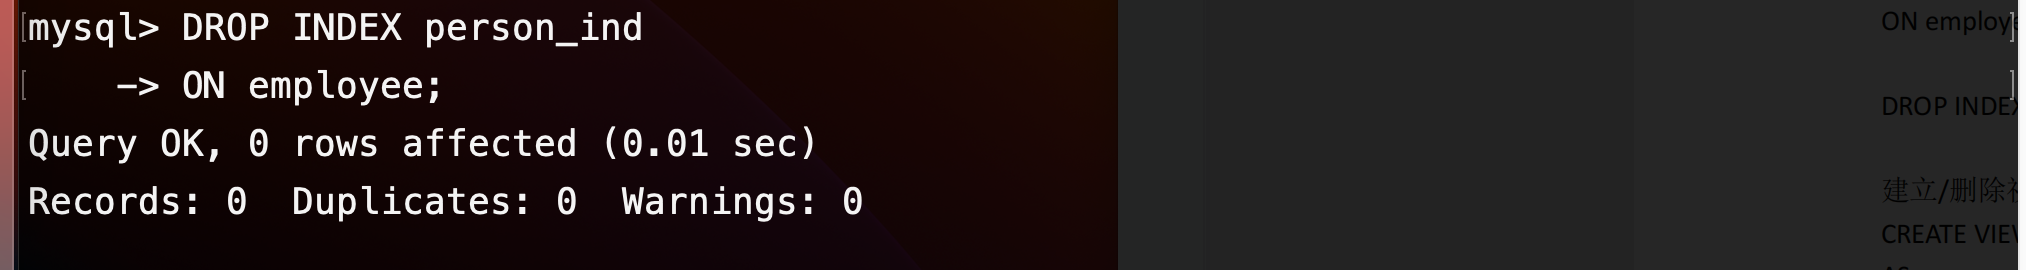
\includegraphics[width=1\textwidth]{lab2/4.png}
        \end{figure}


\subsection*{建立/删除视图}

创建并且删除视图的过程如下

\begin{figure}[H]
        \centering
        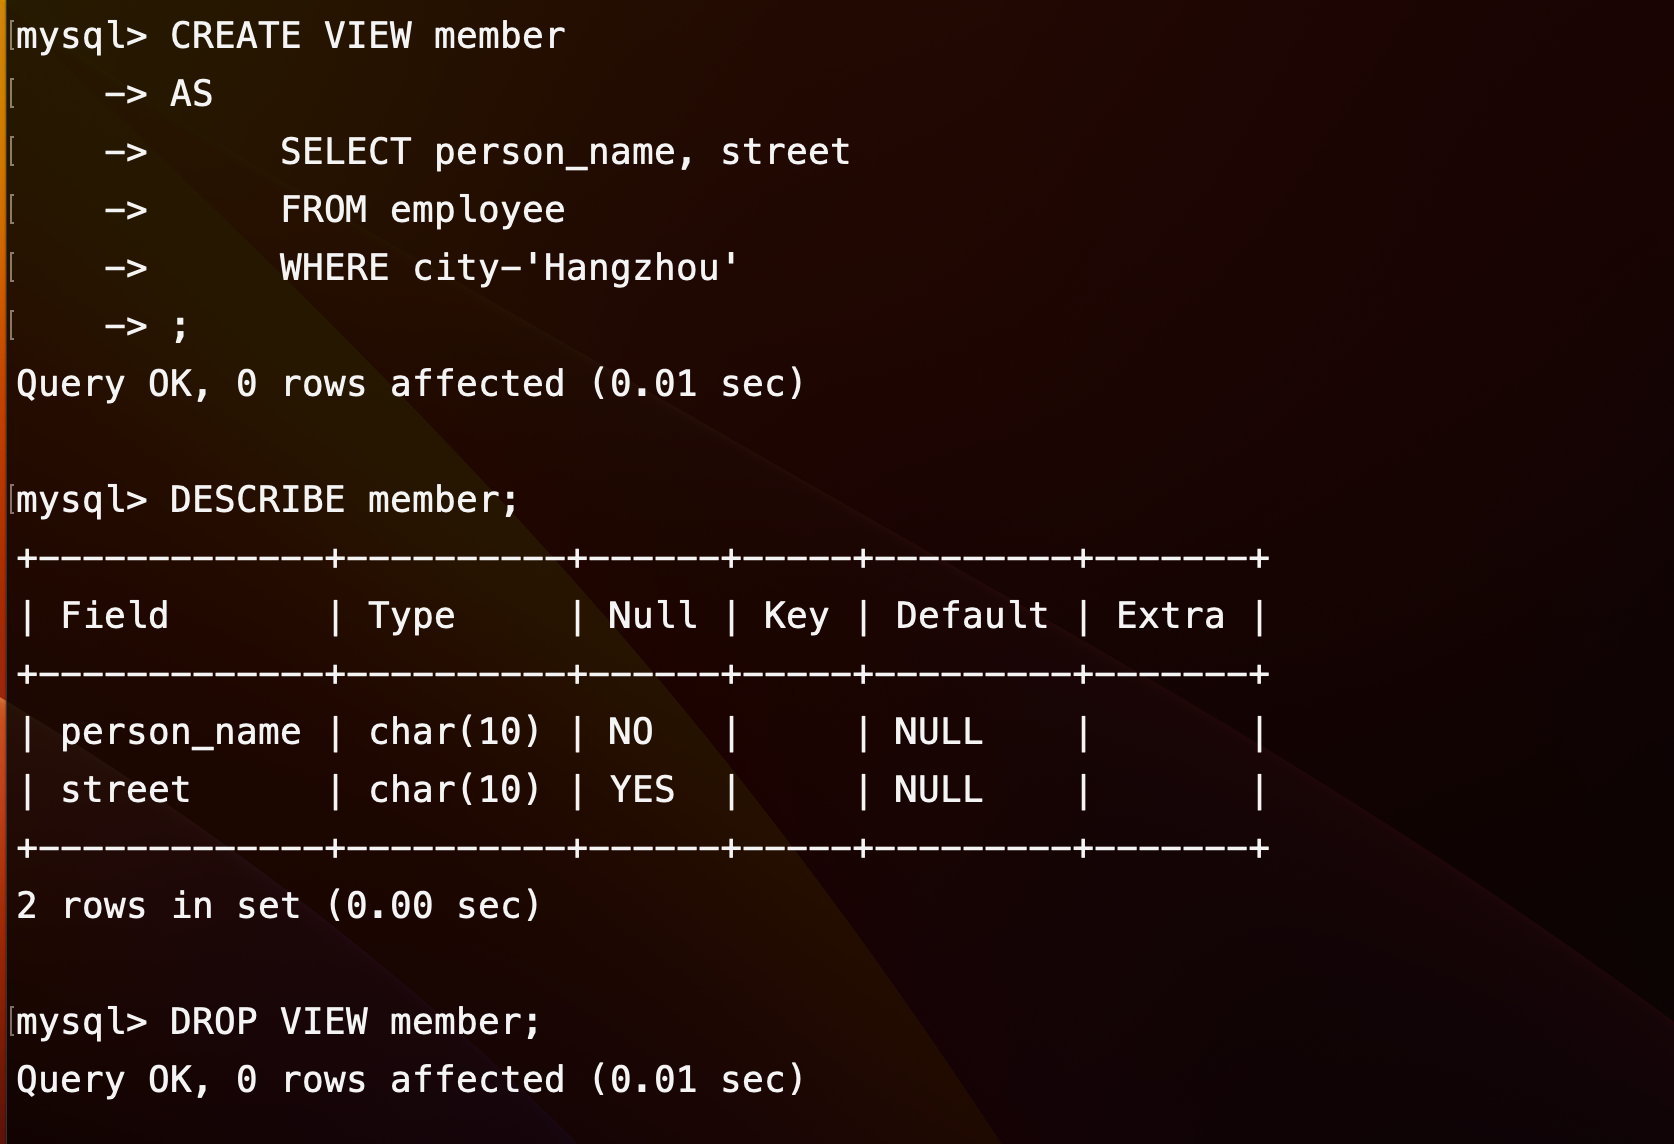
\includegraphics[width=1\textwidth]{lab2/5.png}
        \end{figure}


\subsection*{插入/修改/删除数据}

进行数据的插入

\begin{figure}[H]
    \centering
    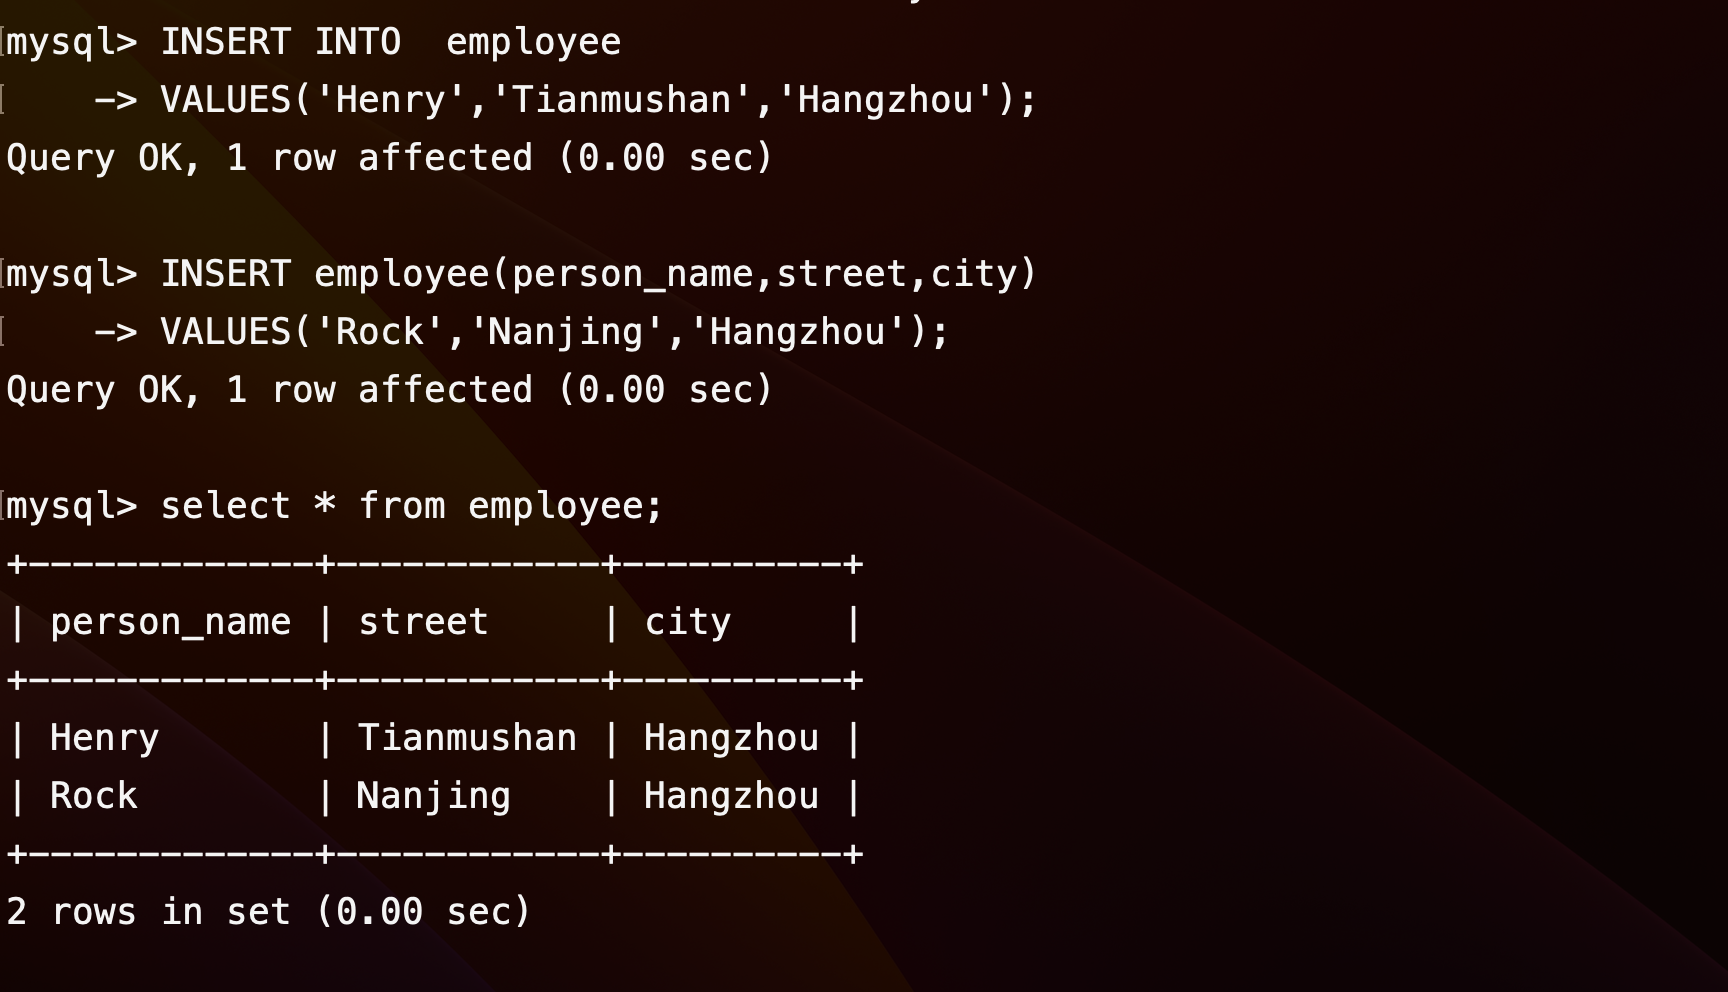
\includegraphics[width=1\textwidth]{lab2/6.png}
    \end{figure}


进行数据的删除
\begin{figure}[H]
    \centering
    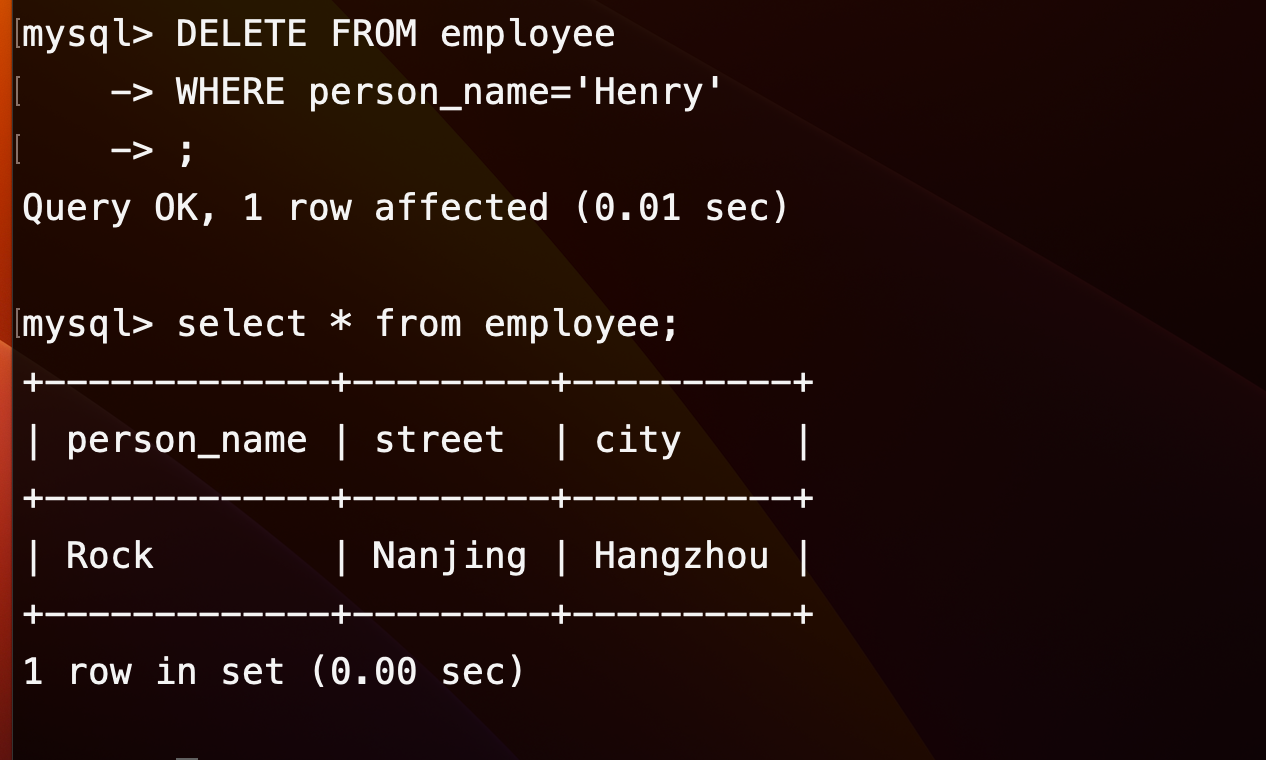
\includegraphics[width=1\textwidth]{lab2/7.png}
    \end{figure}

进行数据的修改

\begin{figure}[H]
    \centering
    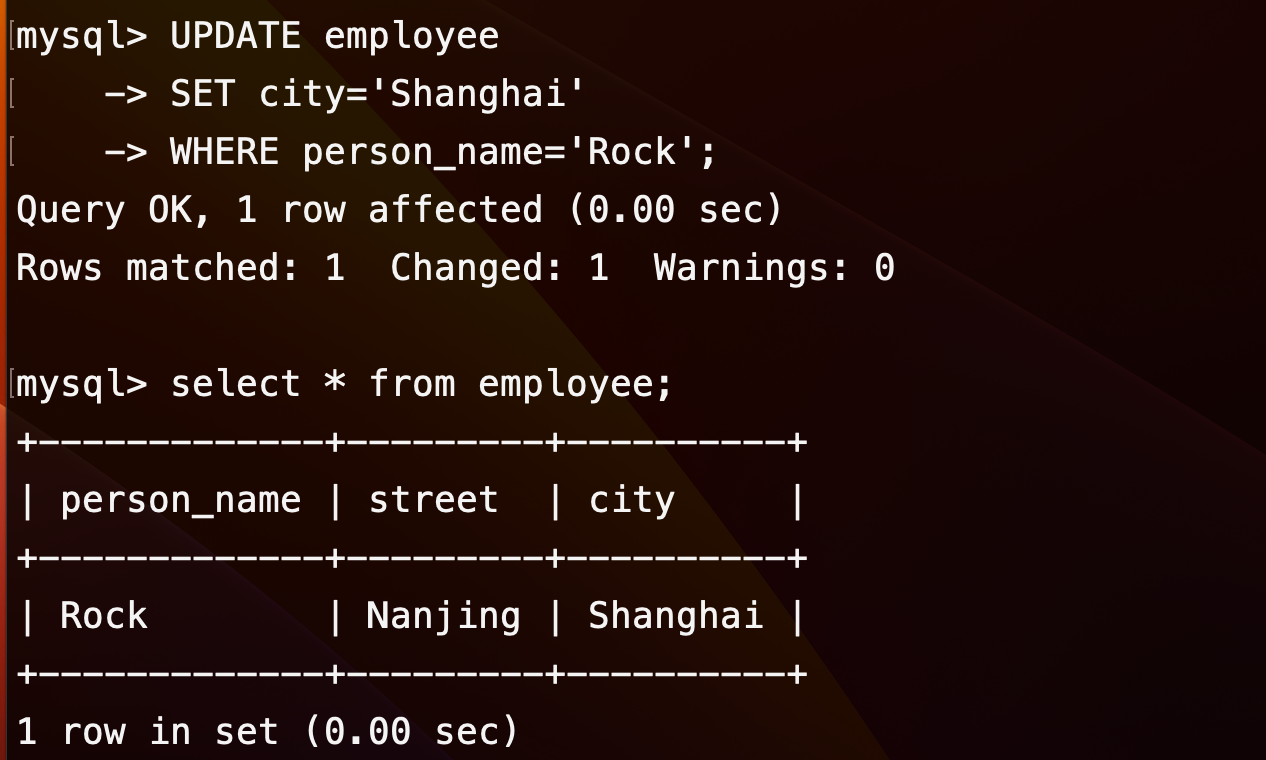
\includegraphics[width=1\textwidth]{lab2/8.png}
    \end{figure}

\subsection*{单表查询}

单表查询操作的过程如下

\begin{figure}[H]
    \centering
    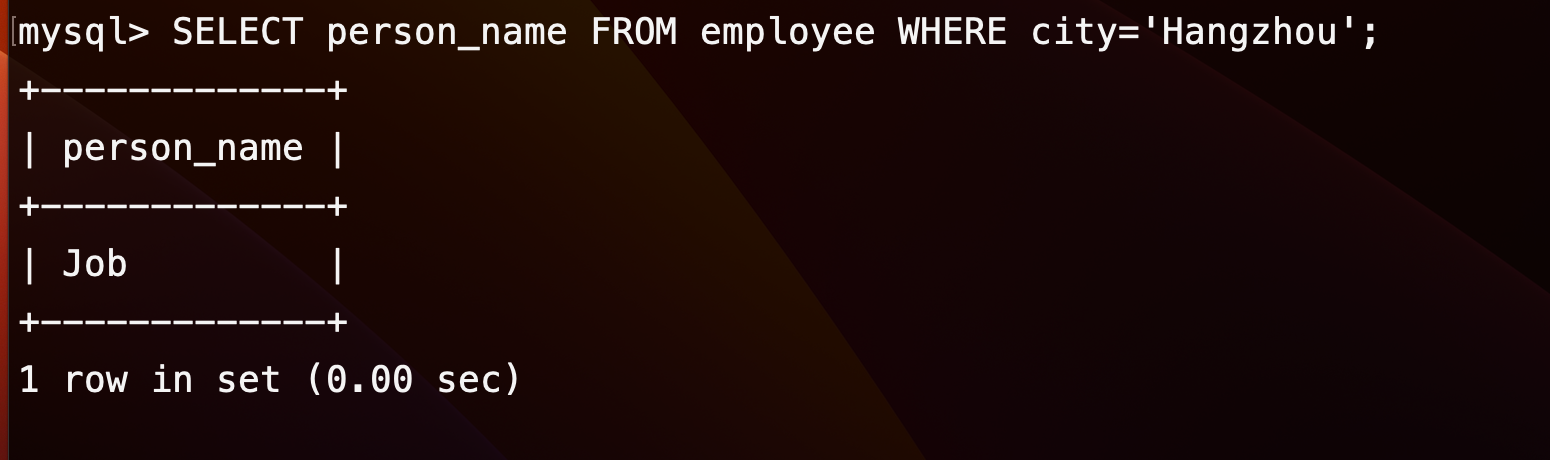
\includegraphics[width=1\textwidth]{lab2/9.png}
    \end{figure}

\subsection*{多表查询}

多表查询的操作如下

\begin{figure}[H]
    \centering
    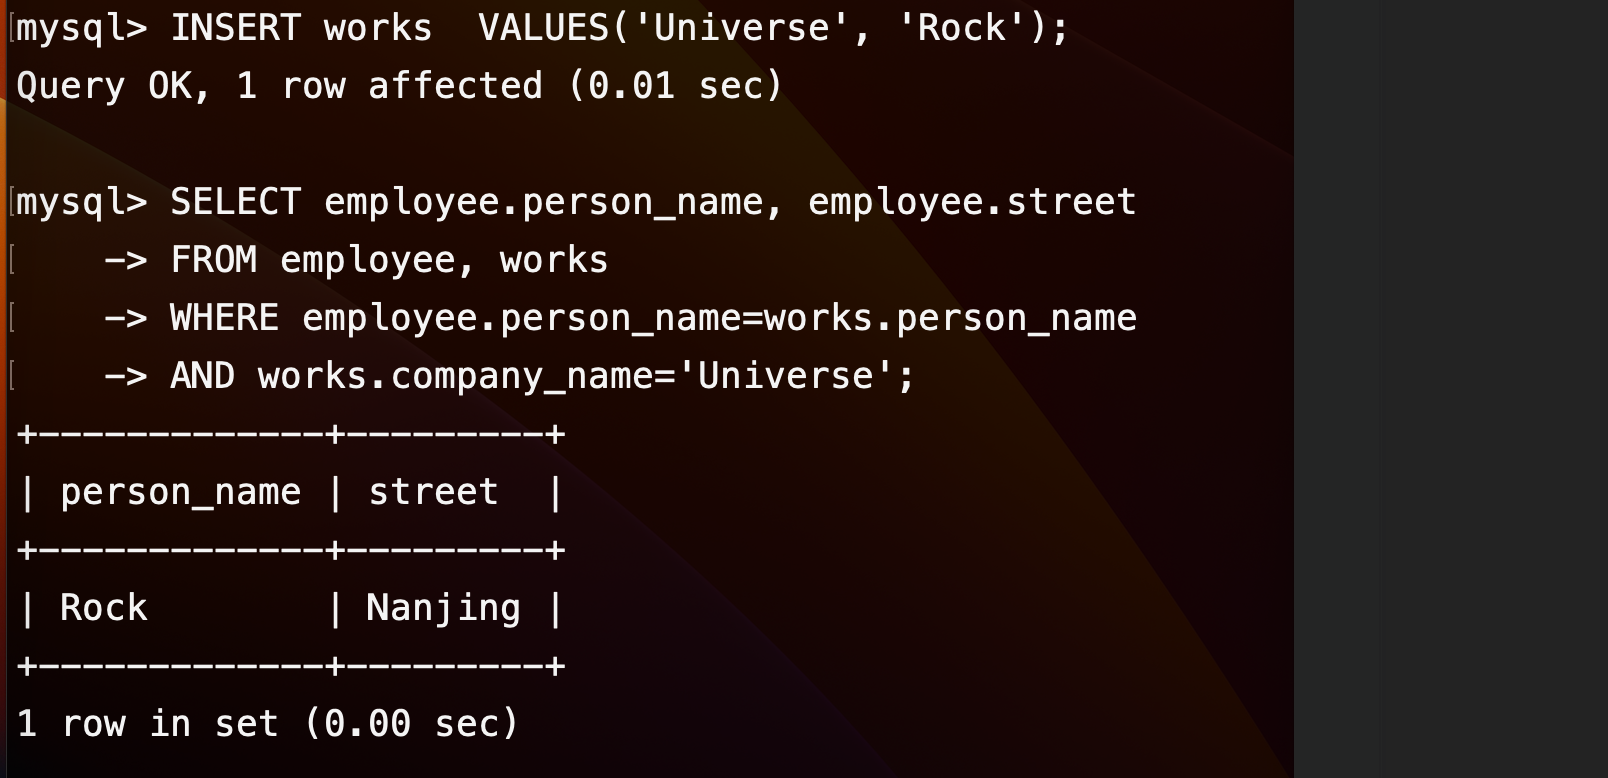
\includegraphics[width=1\textwidth]{lab2/10.png}
    \end{figure}

\subsection*{嵌套子查询}


嵌套查询的操作如下

\begin{figure}[H]
    \centering
    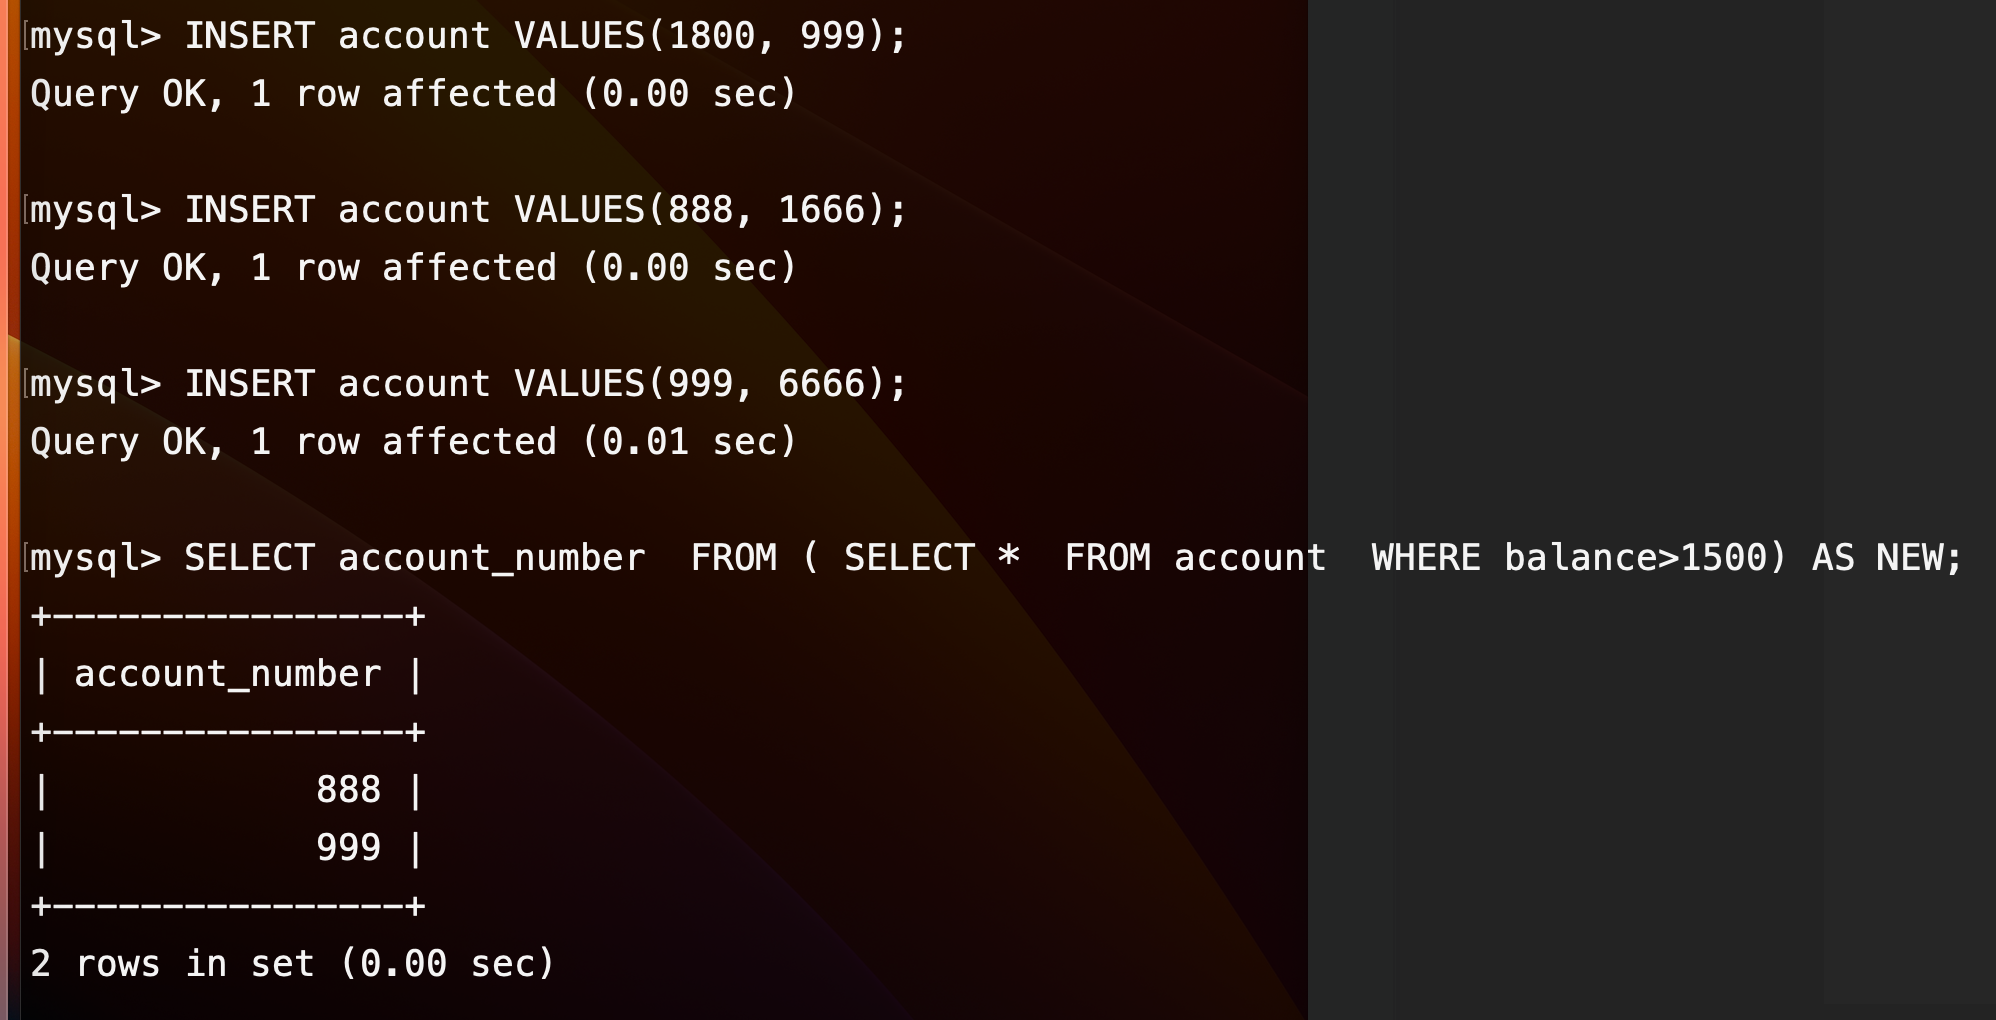
\includegraphics[width=1\textwidth]{lab2/11.png}
    \end{figure}


\subsection*{视图操作}

创建一个新的视图,并且进行数据的查找和修改,过程如下

\begin{figure}[H]
    \centering
    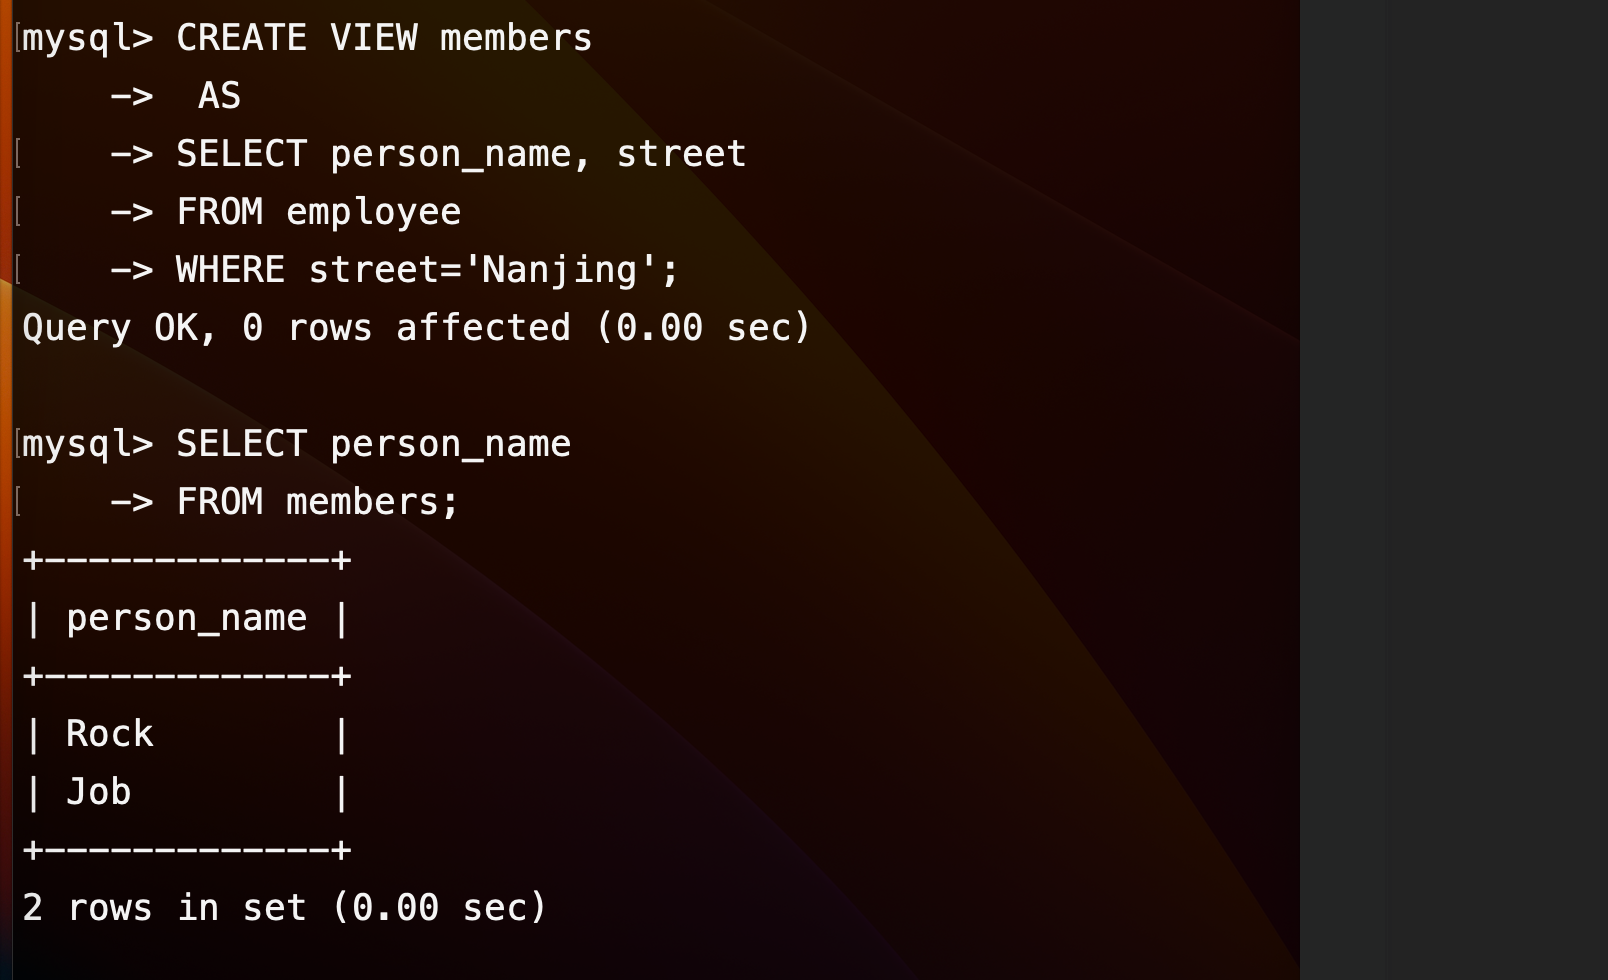
\includegraphics[width=1\textwidth]{lab2/12.png}
    \end{figure}

    \begin{figure}[H]
        \centering
        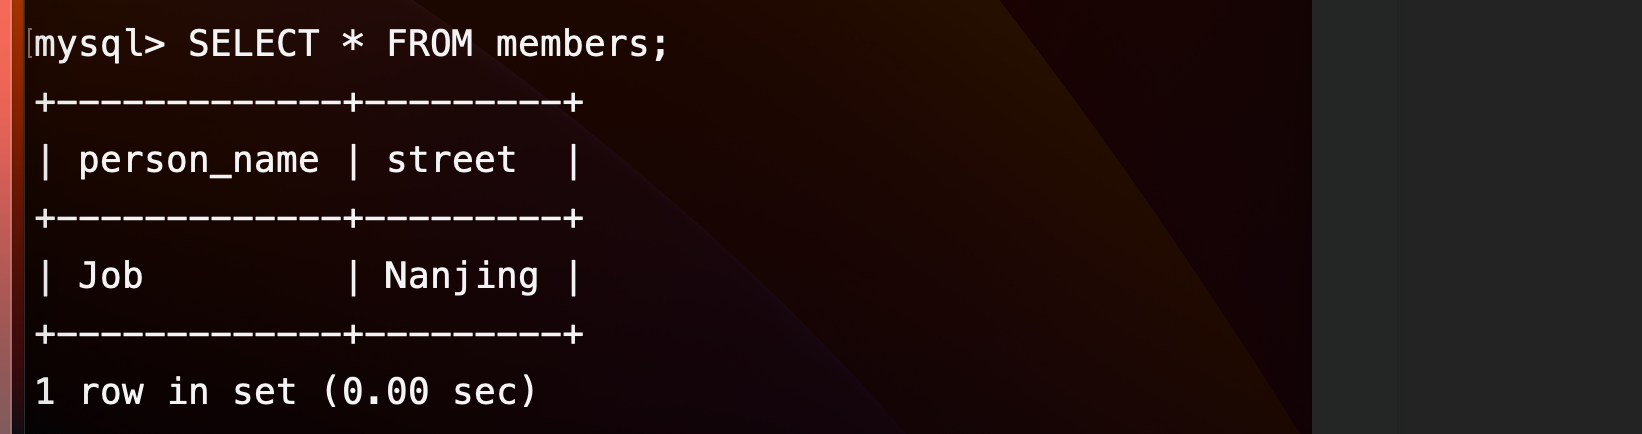
\includegraphics[width=1\textwidth]{lab2/13.png}
        \end{figure}

        \begin{figure}[H]
            \centering
            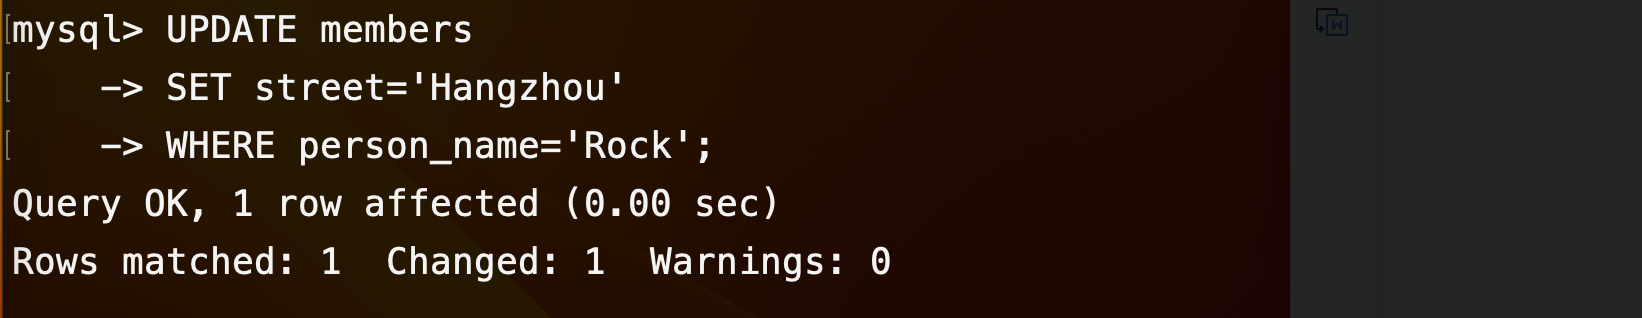
\includegraphics[width=1\textwidth]{lab2/14.png}
            \end{figure}

\end{document}